\documentclass[professionalfonts, xcolor={usenames,svgnames,x11names,table}]{beamer}

\usetheme{SBUclass}
\usepackage{mypackages}
\usepackage{mycommands}


\title{Spell Checking}
\author{Thomas Graf}
\institute{Stony Brook University\\\texttt{lin220@thomasgraf.net}}
\date{LIN 220, Spring 2019\\Lecture 3}


\begin{document}
\unnumbered{
\begin{frame}
	\titlepage
\end{frame}
}

\begin{frame}{Where we are so far\ldots}
    \begin{itemize}
        \item n-grams for word completions
        \item use frequencies to pick most likely completion
        \item prefix trees as efficient storage and search
        \item It's not linguistically perfect,\\
              but it does well enough.
    \end{itemize}

    \begin{block}{One big problem}
        \visible<2>{What if the user made a typo?}
    \end{block}
\end{frame}

\begin{frame}{Spell checking: A naive solution}
    \begin{itemize}
        \item word list (e.g.~stored as prefix tree)
        \item spell checking = lookup in word list
            \begin{itemize}
                \item word found $\Rightarrow$ spelled correctly
                \item word not found $\Rightarrow$ spelled incorrectly
            \end{itemize}
        \item But this simple model is \highlight{not good enough}.
    \end{itemize}

    \pause
    \begin{block}{Open issues}
        \begin{itemize}
            \item How do we determine the correct spelling of a mistyped word?
            \item Not all misspellings are easy to detect.
            \item What if a correctly spelled word is not in the dictionary?\\
                \subpoint{specialized terminology, proper names, neologisms, slang, loan words, \ldots}
        \end{itemize}
    \end{block}
\end{frame}

\begin{frame}{Assessing the problem}
    \begin{itemize}
        \item Never type a single line of code\\
              before you understand the problem!
        \item Think about the \highlight{parameters of the problem}.
        \item Solving the wrong problem is pointless.
    \end{itemize}
    %
    \pause
    \begin{block}{Parameters of the spell checking problem}
        \begin{itemize}
            \item How is the spell checker to be used?\\
                \subpoint{automatic\slash auto correction VS interactive\slash suggestions to user}
            \item What types of misspellings are there?
            \item Is it feasible to detect all of them?
            \item Once we know what the tool should handle,\\
                what is the simplest solution?
        \end{itemize}
    \end{block}
\end{frame}

\begin{frame}{A typology of spelling mistakes}
    \begin{itemize}
        \item \textbf{Cause}\\
            accidental typo $\Leftrightarrow$ unawareness of correct spelling
        \item \textbf{Number}\\
            single-error $\Leftrightarrow$ multi-error
        \item \textbf{Error type}
            \begin{description}
                \item[split] illicit space\\
                    \subpoint{quin tuplets, the set up, atoll way}
                \item[run-on] missing space\\
                    \subpoint{nightvision, boothbabe, atoll way}
                \item[non-word] typed word does not exist\\ 
                    \subpoint{warte or tawer for water}
                \item[real-word] misspelling yields existing word(s) of English\\
                    \subpoint{car toon, it's VS its, their VS there, book for brook, atoll way}
            \end{description}
    \end{itemize}
\end{frame}

\begin{frame}{A difficulty hierarchy of tasks}
    \begin{itemize}
        \item Both typos and spelling confusion can be very hard.
            \begin{itemize}
                \item \emph{labelled} for \emph{labeled}: easy
                \item \emph{awter} for \emph{water}: easy
                \item \emph{nitch} for \emph{niche}: tricky
                \item \emph{awre} for \emph{water}: tricky
            \end{itemize}
        \item Single-error $<$ multi-error
        \item Non-word errors $<$ real-word errors
        \item Difficulty of real-word errors scales with complexity of context:
            \begin{enumerate}
                \item local syntactic configuration
                \item non-local syntactic configuration
                \item word meaning
                \item discourse\slash cross-sentence
                \item world knowledge
            \end{enumerate}
    \end{itemize}
\end{frame}

\begin{frame}{Examples of increasing context complexity}
    \begin{itemize}
        \item \textbf{Local syntactic configuration}\\
              \emph{\colored{purple}{Their} \colored{teal}{are} some biscuits on the counter.}
        \item \textbf{Non-local syntactic configuration}\\
              \emph{\colored{teal}{The man} sitting at the bar \colored{purple}{seem} to be enjoying the atmosphere.}
        \item \textbf{Word meaning}\\
              \emph{We still have to pay off the mortgage on our \colored{purple}{mouse}.}
        \item \textbf{Discourse}\\
              \emph{It's like that time they canceled Futurama. I was so \colored{purple}{bad}.}
        \item \textbf{World knowledge}\\
              \emph{This course is taught at Stony \colored{purple}{Book} University.}
    \end{itemize}
\end{frame}

\begin{frame}{Proper names are impossibly hard}
    \begin{columns}
        \column{.4\linewidth}
        \centering
        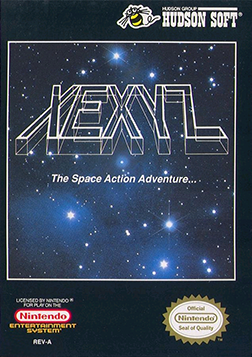
\includegraphics[height=12em]{./img/xexyz}
        \visible<2->{\textbf{Xexyz}}
        \column{.4\linewidth}
        \centering
        
\includegraphics[height=12em]{./img/mxyzptlk}\\
        \visible<3>{\textbf{Mister Mxyzptlk}}
    \end{columns}
\end{frame}

\begin{frame}{How much can we handle efficiently?}
    \begin{itemize}
        \item Always remember:\\
            meaning is hard, world knowledge nigh impossible.
        \item Even non-local syntactic configurations are difficult. 
        \item So we consider only models that handle at most\\
            \highlight{local syntactic configurations}.
    \end{itemize}
\end{frame}

\begin{frame}{$n$-Grams handle local context}
    \begin{itemize}
        \item $n$-gram models can easily detect local real-word errors.
    \end{itemize}
    %
    \begin{example}
        \begin{itemize}
            \item English sentences rarely contain the bigram \emph{their are}.
            \item Hence instances of \emph{their are} are misspellings.
        \end{itemize}
    \end{example}
    %
    \pause
    \textbf{Problems:}
    \begin{itemize}
        \item False positive: incorrectly flags correct words\\
              if they're not in our word list
        \item Sparse data problem all over again.
        \item How do we go from detecting likely errors to\\
              finding likely corrections?
        \item For automatic spell checker, what about cases like\\
              \emph{the man are}?\\
              \subpoint{change \emph{man} to \emph{men} VS change \emph{are} to \emph{is}}
    \end{itemize}
\end{frame}

\begin{frame}{Unlisted words are inevitable}
    \begin{itemize}
        \item No word list can ever contain all words of English.
        \item It is also \highlight{undesirable}:
            \begin{itemize}
                \item No speaker knows or uses all words of English.
                \item Suppose John knows only 10\% of the words in our list.\\
                      Then John will make non-word errors that are real-word errors for the model.
                \item \textbf{Bottom line}\\
                      A big word list \highlight{makes finding misspellings harder}. 
            \end{itemize}
    \end{itemize}
    %
    \pause
    \begin{example}
        \begin{itemize}
            \item Computer scientists use the special term \emph{memoize}.
            \item But for most people \emph{memoize} is a misspelling of \emph{memorize}.
            \item If the dictionary contains \emph{memoize},\\
                then the model will perform \textbf{worse}
                for the majority of users.
        \end{itemize}
    \end{example}
\end{frame}

\begin{frame}{What does ``hard'' mean?}
    \begin{itemize}
        \item A problem is hard if it is difficult to\\
              design a model that performs well on the task.
        \item But what does it mean to perform well?\\
              Detecting both \textbf{\textcolor{blue!75}{positives}} and \highlight{negatives}!\\
    \end{itemize}

    \begin{center}
        \begin{tikzpicture}
            \matrix (m) at (0,0) [matrix of nodes, ampersand replacement=\&] {%
                              \& \textbf{bad} \& \textbf{good}\\
                \textbf{bad} \& true positive \& false negative\\
                \textbf{good}  \& false positive \& true negative\\
                };
                \node [left=0em of m-2-1.south west] (spelling) {Spelling is:};
                \node [above right=0em and -1.25em of m-1-2.north east] (model) {Model says:};

            \begin{pgfonlayer}{background}
                \fill[brown!25] (m-3-2.south west) -| (spelling.south west) -- (spelling.north west) |- (m-2-2.north west) -- cycle;
                \fill[SeaGreen4!25] (m-3-2.north west) |- (model.north west) -- (model.north east) -| (m-2-3.north east) -- cycle;
                \fill[blue!25] (m-3-2.south west) rectangle (m-2-3.north east);
                \foreach \Start/\End/\Color in {%
                    2-2/2-3/blue!25,
                    2-3/2-3/red!50,
                    3-2/3-3/purple!50,
                    3-3/3-3/blue!25}
                    \fill[\Color] (m-\Start.north west) rectangle (m-\End.south east);
            \end{pgfonlayer}
        \end{tikzpicture}
    \end{center}

    \begin{itemize}
        \item Like in medical tests, \textbf{\textcolor{blue!75}{positive}} does not mean ``good''.
        \item For spellchecking: \textbf{\textcolor{blue!75}{positive}} = is a misspelled word
    \end{itemize}
\end{frame}

\begin{frame}{Precision and Recall}
    There are two measures of model performance:

    \begin{description}
        \item[Precision] How many posited positives are actual positives?
        \item[Recall]    How many of the actual positives are\\
                         recognized as positives?
    \end{description}
    
    \begin{block}{Formal definition}
        \begin{align*}
            \text{Precision}
                &= \frac{%
                         \text{\color{blue!75}true positives}}{%
                         \text{\textcolor{blue!75}{true positives} +
                               \textcolor{purple!75}{false positives}}
                         }
                = \frac{\text{\color{blue!75}true positives}}{\text{all posited positives}}\\
                \\
            \text{Recall}
                &= \frac{%
                         \text{\color{blue!75}true positives}}{%
                         \text{\textcolor{blue!75}{true positives} +
                               \textcolor{red!75}{false negatives}}
                         }
                = \frac{\text{\color{blue!75}true positives}}{\text{all actual positives}}\\
        \end{align*}
    \end{block}
\end{frame}

\begin{frame}{A calculation example}
    Our spellchecker performs as follows over 100 words:

    \begin{columns}
        \column{.5\linewidth}
        \begin{center}
            \begin{tabular}{rcc}
                & \textbf{bad} & \textbf{good}\\
                \textbf{bad} & 25 & 10\\
                \textbf{good} & 30 & 35\\
            \end{tabular}
        \end{center}

        \column{.5\linewidth}
        \begin{enumerate}
            \item \textcolor{blue!75}{True positives}: \visible<2->{\textcolor{blue!75}{25}}
            \item \textcolor{blue!75}{True negatives}: \visible<3->{\textcolor{blue!75}{35}}
            \item \textcolor{purple!75}{False positives}: \visible<4->{\textcolor{purple!75}{30}}
            \item \textcolor{red!75}{False negatives}: \visible<5->{\textcolor{red!75}{10}}
        \end{enumerate}
    \end{columns}

    \visible<6->{%
    \begin{align*}
        \text{Precision}
            &= \frac{%
                     \text{\textcolor{blue!75}{%
                           \only<6>{true positives}
                           \only<7->{25}
                           }}}{%
                     \text{\textcolor{blue!75}{%
                           \only<6,7>{true positives}
                           \only<8->{25}
                           } +
                           \textcolor{purple!75}
    \end{align*}}

    \medskip
    \visible<11->{%
    \begin{align*}
        \text{Recall}
            &= \frac{%
                     \text{\textcolor{blue!75}{%
                           \only<11>{true positives}
                           \only<12->{25}
                           }}}{%
                     \text{\textcolor{blue!75}{%
                           \only<11,12>{true positives}
                           \only<13->{25}
                           } +
                           \textcolor{red!75}
    \end{align*}
    }
\end{frame}

\begin{frame}{The abstract principle}
    \begin{example}
        A large word list
        \begin{itemize}
            \item \visible<2->{increases} precision: \visible<3->{correct spellings are less likely to be flagged as incorrect}
            \item \visible<4->{decreases} recall: \visible<5->{non-word errors by the user\\ are incorrectly treated as correct spellings}
        \end{itemize}
    \end{example}

    Precision and recall are quantitative counterparts to\\
    soundness and completeness:

    \begin{description}
        \item[sound] If the model says X is a positive, then X is a positive.
        \item[complete] If X is a positive, then the model says X is a positive.
    \end{description}
\end{frame}

\begin{frame}{``I still don't get it!''}
    Here's the simplistic version:

    \begin{description}
        \item[low precision] many actual negatives are misclassified as positives;\\
                             the model is too eager to find positives
        \item[low recall]    many actual positives are misclassified as negatives;\\
                             the model misses too many positives
    \end{description}
\end{frame}

\begin{frame}{Interim summary}
    \textbf{Precision and recall}
    \begin{itemize}
        \item ``Performing well'' is too vague a notion.
        \item In order to evaluate models, we need more rigorous metrics.
        \item Precision and recall allow us to quantify performance\\
              along two important axes.
    \end{itemize}

    \textbf{Spelling}
    \begin{itemize}
        \item We want to handle at least non-word errors.
        \item We want to handle at most local syntactic real-word errors.
        \item We want to be able to detect and suggest corrections.
        \item A word list of all English words is impossible.
        \item It is undesirable because it greatly lowers precision.
    \end{itemize}
\end{frame}

\begin{frame}{A cool idea that is hard to realize}
    \begin{itemize}
        \item One conceivable solution is to \highlight{stratify} the dictionary into
            \begin{itemize}
                \item a base vocabulary used by all English speakers, and
                \item optional extensions for specific genres, styles, etc.
            \end{itemize}
        \item Extensions could be loaded if the text so far\\
              fits certain criteria.\\
            \subpoint{high number of field-specific terms, loan words, etc.}
        \item To the best of my knowledge,\\
              nobody has ever tried anything like this.
        \item The payoff probably isn't worth the effort.\\
              So what's the \highlight{alternative?}
    \end{itemize}
\end{frame}

\begin{frame}{Another Solution for Unlisted Words}
    \begin{itemize}
        \item Humans can easily distinguish possible words of English\\
            from impossible ones.
    \end{itemize}
    %
    \begin{example}
        \begin{center}
            \begin{tabular}{c@{\hspace{2em}}c}
                \textbf{possible} & \textbf{impossible}\\
                blick & bnick\\
                wrexel & rwexel\\
                lakoo & ooakl\\
                orcalate & orclte
            \end{tabular}
        \end{center}
    \end{example}
    %
    \begin{itemize}
        \item Only some sequences of characters can occur in English words.
        \item You guessed it: \highlight{n-grams again!}
    \end{itemize}
\end{frame}

\begin{frame}{Character $n$-grams for non-word detection}
    \textbf{Non-word detection algorithm}
    \begin{enumerate}
        \item Compile list of character bigrams\\
              that occur in words in the word list.
        \item A word is a non-word if it
            \begin{enumerate}
                \item is not in the dictionary, and
                \item contains an illicit character bigram
            \end{enumerate}
    \end{enumerate}

    \begin{example}
        \begin{itemize}
            \item Word list: bee, bored, doom
            \item Character bigrams: be, ee, bo, or, re, ed, do, oo, om
        \end{itemize}

        \centering
        \begin{tabular}{rccc}
            \toprule
            \textbf{Word} & \textbf{In list?} & \textbf{Illicit bigram?} & \textbf{Verdict?}\\            
            \midrule
            bee & yes & --- & good\\
            boredom & no & no & good\\
            bnick & no & yes & bad\\
            beeeereed & no & no & good\\
            \bottomrule
        \end{tabular}
    \end{example}
\end{frame}

\begin{frame}{Which impossible words are detected?}
    \begin{itemize}
        \item We have seen several times by now that\\
              bigrams are insufficient in certain applications. 
        \item We can increase the value of $n$ (e.g.~3, 4, 5).
    \end{itemize}
    %
    \begin{example}
        \centering
        \begin{tabular}{rcl}
            \textbf{Impossible Word} & \textbf{Character Bigrams} & \textbf{Illicit Bigrams}\\
            \hline
            bnick & bn, ni, ic, ck & bn\\
            rwexel & rw, we, ex, xe, el & \textbf{none!}\\
            akklaim & ak, kk, kl, la, ai, im & \textbf{none!}\\ 
        \end{tabular}
    \end{example}
\end{frame}

\begin{frame}{Improving the $n$-gram model}
    \begin{enumerate}
        \item \textbf{Size}
            \begin{itemize}
                \item trigrams much better than bigrams
                \item \emph{Example}\\
                    \emph{kk} and \emph{kl} occur in a few English words, but not \emph{kkl}
            \end{itemize}
        \item \textbf{End Markers}
            \begin{itemize}
                \item beginning and end of English words are special
                \item \emph{Examples}\\
                    \emph{nk} is very common, but impossible at beginning of word\\
                    \emph{cl} is very common, but impossible at end of word
                \item special character \$ for word edges\\
                    \subpoint{\emph{\$nk} impossible, \emph{nk} and \emph{nk\$} allowed}
            \end{itemize}
        \item \textbf{Probabilities}
            \begin{itemize}
                \item determine frequency of character $n$-grams
                \item treat non-word probability as product of character $n$-grams
                \item everything below a certain threshold is a non-word
            \end{itemize}
    \end{enumerate}
\end{frame}

\begin{frame}{Finding the correct word}
    \begin{itemize}
        \item We have word $n$-grams for\\
              finding some instances of real-word errors.
        \item We have word lists and character $n$-grams for\\
              finding non-word errors.
        \item \textbf{But:} still need mechanism for \highlight{spelling suggestions}.
        \item \textbf{Three Common Approaches}
            \begin{itemize}
                \item rule-based
                \item similarity key
                \item minimum edit distance
            \end{itemize}
    \end{itemize}
\end{frame}

\begin{frame}{Option 1: Ruled-based approach}
    \begin{itemize}
        \item custom rules provide candidate lists for specific misspellings
    \end{itemize}
    %
    \begin{example}
        \begin{itemize}
            \item teh $\Rightarrow$ the
            \item refering $\Rightarrow$ referring
            \item fyre $\Rightarrow$ fire, fry
        \end{itemize}
    \end{example}
    %
    \begin{itemize}
        \item can be collected by hand or automatically
    \end{itemize}
    %
    \pause
    \begin{center}
        \begin{tabular}{ll}
            \textbf{Advantages} & \textbf{Disadvantages}\\
            conceptually simple & labor intense\\
                                & inflexible
        \end{tabular}
    \end{center}
\end{frame}

\begin{frame}{Option 2: Similarity keys}
    \begin{itemize}
        \item classify strings of characters according to similarity
        \item words in same similarity class are offered as suggestions
    \end{itemize}
    %
    \begin{exampleblock}{Example: US Census Soundex Algorithm}
        \begin{columns}
            \column{.75\linewidth}
            \begin{enumerate}
                \item Always retain first letter.
                \item Drop all (other) occurrences of \emph{a}, \emph{e}, \emph{i}, \emph{o}, \emph{u}, \emph{y}, \emph{h}, \emph{w}.
                \item Replace all (other) consonsants by digits:
                    \begin{itemize}
                        \item \emph{b}, \emph{f}, \emph{p}, \emph{v} $\Rightarrow$ 1
                        \item \emph{c}, \emph{g}, \emph{j}, \emph{k}, \emph{s}, \emph{x}, \emph{z} $\Rightarrow$ 2
                        \item \emph{d}, \emph{t} $\Rightarrow$ 3
                        \item \emph{l} $\Rightarrow$ 4
                        \item \emph{m}, \emph{n} $\Rightarrow$ 5
                        \item \emph{r} $\Rightarrow$ 6
                    \end{itemize}
                \item Remove consecutive copies of same digit.
                \item Shorten\slash lengthen to 4 characters.
            \end{enumerate}

            \column{.35\linewidth}
            \begin{tabular}{rl}
                \colored{purple}{bearded} &
                \footnotesize $\underrightarrow{1+2}$ \\
                \colored{purple}{brdd} &
                \footnotesize $\underrightarrow{3}$ \\
                \colored{purple}{b633} &
                \footnotesize $\underrightarrow{4}$ \\
                \colored{purple}{b63} &
                \footnotesize $\underrightarrow{5}$ \\
                \colored{purple!50!teal}{b630} &
                \footnotesize $\underleftarrow{5}$    \\
                \colored{teal}{b63} &
                \footnotesize $\underleftarrow{4}$  \\
                \colored{teal}{b663} &
                \footnotesize $\underleftarrow{3}$  \\
                \colored{teal}{brrd} &
                \footnotesize $\underleftarrow{1+2}$  \\
                \colored{teal}{borrowed}
            \end{tabular}
        \end{columns}
    \end{exampleblock}
\end{frame}

\begin{frame}{(Dis)Advantages of similarity keys}
    \textbf{Advantages}
    \begin{itemize}
        \item easy to implement
        \item easy to compute
    \end{itemize}

    \textbf{Disadvantages}
    \begin{itemize}
        \item similarity key must be carefully designed for application\\
            \subpoint{Soundex is not a good choice for spell checking}
        \item may need distinct key for distinct languages
    \end{itemize}
\end{frame}

\begin{frame}{Option 3: Minimum edit distance}
    How many steps does it take to transform one word into another?
    %
    \begin{block}{Levenshtein Distance}
        The Levenshtein Distance between \colored{purple}{x} and \colored{teal}{y} is \colored{orange}{n}\\
        if the shortest sequence of
        %
        \begin{itemize}
            \item single character deletions, and\slash or
            \item single character insertions, and\slash or
            \item single character substitutions
        \end{itemize}
        %
        that turns \colored{purple}{x} into \colored{teal}{y} takes \colored{orange}{n} steps.
    \end{block}
    %
    \begin{exampleblock}{Example: Transforming \emph{meat} into \emph{bats}}
        \centering
        \begin{tabular}{rl}
            \textbf{String} & \textbf{Operation}\\
            meat & \\
            beat & substitute \emph{b} for \emph{m}\\
            bat  & delete \emph{e}\\
            bats & insert \emph{s}
        \end{tabular}
    \end{exampleblock}
\end{frame}

\begin{frame}{Computing Levenshtein distances}
    \begin{itemize}
        \item The Levensthein distance is determined by\\
              the \highlight{shortest sequence} of operations.
        \item How do we know that there isn't a shorter solution?
    \end{itemize}    

    \begin{block}{Naive Solution}
        \begin{itemize}
            \item Try all possible 1-step sequences.
            \item If desired word among outputs, Levenshtein distance is 1.
            \item Otherwise, try all 2-step sequences.
            \item If desired word among outputs, Levenshtein distance is 2.
            \item Otherwise, \ldots
        \end{itemize}
    \end{block}
\end{frame}

\begin{frame}{Evalutating the naive solution}
    \begin{itemize}
        \item The naive solution is guaranteed to terminate\\
              (= it won't run forever).
        \item \textbf{Reason:} The Levenshtein distance between two words is\\
            at most the length of the longer word.
        \item \textbf{But:} The \highlight{combinatorial explosion} is enormous.
    \end{itemize}
    %
    \begin{example}
        4 character word, 26 letter alphabet

        \medskip
        \centering
        \begin{tabular}{rll}
            \textbf{Steps} & \textbf{Possible Operations} & \textbf{Computed Strings}\\
            1 & $4$ del, $5 \times 26$ ins, $4 \times 26$ sub& 238\\
            2 & $10$ del, $15 \times 26$ ins, $10 \times 26$ sub& 660\\
        \end{tabular}
    \end{example}
\end{frame}

\begin{frame}{Improving efficiency}
    \begin{itemize}
        \item \textbf{Problem 1:} ``generate and test'' is too undirected
        \item \textbf{Problem 2:} $n$-step calculation repeats computations from $(n-1)$-step calculation
    \end{itemize}
    %
    \begin{block}{Dynamic Programming}
        \begin{enumerate}
            \item Decompose big problems into small problems.
            \item Solve the small problems and \highlight{save the solution}.
            \item Look up stored solutions rather than recomputing them.
        \end{enumerate}

        \textbf{Intuition:} Write down intermediate results, just like humans do.
    \end{block}
\end{frame}

\begin{frame}{Dynamic programming for Levenshtein distance}
    \begin{itemize}
        \item Draw a graph that represents the possible edit sequences\\
              from \colored{purple}{x} to \colored{teal}{y}.
        \item We want the least costly path through that graph.
        \item Dynamic programming solution:
            \begin{enumerate}
                \item For each node,\\
                      what is the least costly path to it from adjacent nodes?
                \item Throw away all other paths.
                \item Go backwards from target to source to find correct path.
            \end{enumerate}
    \end{itemize}
\end{frame}

\begin{frame}{Example of dynamic programming}
    \begin{center}
        \begin{tikzpicture}
            \foreach \x in {0,...,4}
                \foreach \y in {0,...,3}
                    {
                    \pgfmathtruncatemacro{\label}{\x + 5 * \y + 1}
                    \node[circle, draw=blue!50, fill=blue!50, minimum size=2em] (\x\y) at (5*\x em, -5*\y em) {\label};
                    }

            % arcs
            \foreach \Source/\Target/\Label/\Orient/\Time in {%
                    00/01/1/right/2-,
                    00/10/1/below/2-,
                    00/11/0/right/2-,
                    10/20/1/below/2-,
                    10/11/1/right/2-5,
                    10/21/1/right/2-7,
                    20/30/1/below/2-,
                    20/21/1/right/2-7,
                    20/31/1/right/2-9,
                    30/40/1/below/2-,
                    30/31/1/right/2-9,
                    30/41/1/right/2-11,
                    40/41/1/right/2-11,
                    01/11/1/below/2-5,
                    01/02/1/right/2-,
                    01/12/1/right/2-13,
                    11/12/1/right/2-,
                    11/21/1/below/2-,
                    11/22/1/right/2-,
                    21/31/1/below/2-,
                    21/22/1/right/2-14,
                    21/32/0/right/2-,
                    31/41/1/below/2-,
                    31/32/1/right/2-15,
                    31/42/1/right/2-16,
                    41/42/1/right/2-16,
                    02/12/1/below/2-13,
                    02/03/1/right/2-,
                    02/13/1/right/2-18,
                    12/22/1/below/2-14,
                    12/13/1/right/2-,
                    12/23/0/right/2-,
                    22/32/1/below/2-15,
                    22/23/1/right/2-19,
                    22/33/1/right/2-,
                    32/42/1/below/2-,
                    32/33/1/right/2-,
                    32/43/1/right/2-,
                    42/43/1/right/2-21,
                    03/13/1/below/2-18,
                    13/23/1/below/2-19,
                    23/33/1/below/2-,
                    33/43/1/below/2-21%
                }
                {
                \draw[->, visible on=<\Time>] (\Source) to node [\Orient, pos=.7] {\Label} (\Target);
                }

            % node costs
            \foreach \Node/\Label/\Time in {
                    00/0/3-,
                    10/1/4-,
                    01/1/5-,
                    11/0/6-,
                    20/2/7-,
                    21/1/8-,
                    30/3/9-,
                    31/2/10-,
                    40/4/11-,
                    41/3/12-,
                    02/2/13-,
                    12/1/14-,
                    22/1/15-,
                    32/1/16-,
                    42/2/17-,
                    03/3/18-,
                    13/2/19-,
                    23/1/20-,
                    33/2/21-,
                    43/2/22-%
                }
                \node<\Time>[rectangle, rounded corners, fill=orange!75, opacity=.8, xshift=.25em, yshift=.25em]
                    at (\Node.north east) {\small \Label};



            % spell out fyre
            \foreach \Source/\Target/\Label in {%
                    00/10/f,
                    10/20/y,
                    20/30/r,
                    30/40/e%
                }
                \node at ($(\Source) !.5! (\Target)$) [yshift = 1em] {\color{purple}\Label};

            % spell out fry
            \foreach \Source/\Target\Label in {%
                    00/01/f,
                    01/02/r,
                    02/03/y%
                }
                \node at ($(\Source) !.5! (\Target)$) [xshift = -1em] {\color{teal}\Label};

            \node[draw,circle] (legend-root) at (40) [xshift=3em, yshift=2em] {};
            \node[draw,circle] (legend-insert) [below=4.5em of legend-root] {};
            \node[draw,circle] (legend-delete) [right=4.5em of legend-root] {};
            \node[draw,circle] (legend-substitute) [right=4.5em of legend-insert] {};

            \foreach \Target/\Distance/\Label in {
                    delete/.2/{delete \colored{purple}{x}},
                    insert/.4/{insert \colored{teal}{y}},
                    substitute/.4/{substitute \colored{teal}{y} for \colored{purple}{x}}
                    }
                \draw[->] (legend-root) to node [above=-\Distance em,sloped] {\small \Label} (legend-\Target);

            % fyre start node
            \node (fyre) [above=1em of 00] {fyre};
            \draw[->] (fyre) to (00);

            % fry end node
            \node (fry) [right=1em of 43] {fry};
            \draw[->] (43) to (fry);
        \end{tikzpicture}
    \end{center}
\end{frame}

\begin{frame}{Evaluation of Levenstein distance}
    \begin{itemize}
        \item fully automatic
        \item more easily applied across languages\\
              (given a character-based orthography)
        \item computationally demanding, but
            \begin{itemize}
                \item dynamic programming tames the beast
                \item majority of misspellings have distance $\leq 3$
            \end{itemize}
    \end{itemize}

    \pause
    \begin{block}{Comparsion of Edit Distance Metrics}
        \centering
        \begin{tabular}{ll}
            \textbf{Metric} & \textbf{Operations}\\
            Damerau-Levenshtein & insert, delete, substitute, transpose\\
            Levenshtein & insert, delete, substitute\\
            longest common subsequence & insert, delete\\
            Hamming & substitute
        \end{tabular}
    \end{block}
\end{frame}

\begin{frame}{Adding probabilities$\ldots$ again}
    \begin{itemize}
        \item Once again probabilities improve accuracy.
        \item \textbf{Confusion probabilities} measure how likely\\
            one word is to be typed as realization of another.
        \item Difficult to compute, affected by many parameters\\
            \subpoint{keyboard layout, pronunciation, optical similarity, context, \ldots}
    \end{itemize}
\end{frame}

\begin{frame}{Putting it all together}
    \textbf{Step 1: Detecting Spelling Errors}\\
            \begin{itemize}
                \item \emph{Non-Word Errors}\\
                    %
                    \begin{enumerate}
                        \item Is the word in the dictionary?
                        \item If no, does the word contain illicit character $n$-grams?
                        \item If no, is the word an unlikely combination of licit character $n$-grams?
                    \end{enumerate}
                %
                \item \emph{Real-Word Errors}\\
                    %
                    \begin{enumerate}
                        \item Does the word appear in an illicit $n$-gram?
                        \item If no, does the word appear in an unlikely $n$-gram?
                    \end{enumerate}
            \end{itemize}
\end{frame}

\begin{frame}{Putting it All Together [cont.]}
    \textbf{Step 2: Computing and Ranking Possible Corrections}\\
        \begin{enumerate}
            \item \emph{Calculate Set of All Possible Corrections}
                \begin{itemize}
                    \item just use dictionary
                    \item use naive edit distance algorithm to compute set of possible corrections up to some distance, then remove all words not in dictionary
                \end{itemize}
            %
            \item \emph{Ranking Possible Corrections}\\
                combined heuristic based on
                %
                \begin{itemize}
                    \item Levenshtein distance
                    \item confusion probability
                    \item word probability
                    \item maximizing sentence probability
                \end{itemize}
        \end{enumerate}
\end{frame}

\end{document}

homework
 - generalize bigram list code to n-gram list function
 - non-word detection algorithm given list of illicit n-grams
